\documentclass[conference]{IEEEtran}

% --- Change subsubsection numbering to A.1, A.2, etc. ---
\makeatletter
% 1. How it displays in the heading (A.1, A.2)
\renewcommand{\thesubsubsectiondis}{\Alph{subsection}.\arabic{subsubsection}}

% 2. How it displays when you use \ref{} in text (A.1, A.2)
% (If you prefer \ref{} to still show "III-A.1", leave this next line out)
\renewcommand{\thesubsubsection}{\Alph{subsection}.\arabic{subsubsection}}
\makeatother
% --------------------------------------------------------

\usepackage{amsmath,amssymb,amsfonts}
\usepackage{mathtools}
\usepackage{booktabs}
\usepackage{array}
\usepackage{enumitem}
\usepackage{algorithm}
\usepackage{algorithmic}
\usepackage{graphicx}
%\usepackage[hidelinks]{hyperref}
\usepackage{amsthm}

\usepackage{tabularx}
\usepackage{ragged2e}
\usepackage{booktabs}

\newcommand{\States}{\mathcal{S}}
\newcommand{\Items}{\mathcal{I}}
\newcommand{\Skills}{\mathcal{K}}
\newcommand{\Flags}{\mathcal{F}}
\newcommand{\Assets}{\mathcal{A}}
\newcommand{\Quests}{\mathcal{Q}}
\newcommand{\MainQ}{\mathcal{Q}^{\mathrm{main}}}
\newcommand{\SideQ}{\mathcal{Q}^{\mathrm{side}}}
\newtheorem{definition}{Definition}

\usepackage{xcolor} 
\usepackage{listings}
\usepackage{url}
\input{jsonstyles}
\input{compactspace}

\begin{document}

\title{Verifying Story Continuity During Game Content Evolution with Resource-Annotated Graphs}

\author{Ciprian Paduraru$^{1,2}$, Irina Ciocan$^2$, and Alin Stefanescu$^{2,3}$
% \\ (start a new line for the affiliation block)
\\
\IEEEauthorblockA{$^1$Gameloft}
\IEEEauthorblockA{$^2$University of Bucharest, Romania}
\IEEEauthorblockA{$^3$Institute for Logic and Data Science, Romania}}

\maketitle

\begin{abstract}
Story-driven games can exhibit continuity defects in which players become
blocked from intended progression, reach mandatory content without required
assets, or enter narrative states inconsistent with prior choices. Such
defects are difficult to detect through local testing and are often found
during integration, when diagnosis requires reconstructing long action
sequences across quests and content areas.

This paper presents a framework for verifying story continuity in game
content pipelines using resource-annotated story graphs extracted from
production metadata. The engine-independent analysis core operates on
exported story models and continuity rules, while project-specific
adapters handle content extraction and optional replay. Continuity
expectations are expressed in a lightweight requirements language and
analysed through temporal property checking and graph exploration over
abstract configurations. Reported violations are translated into abstract counterexample traces
that can be replayed on instrumented builds, linking specification
failures to reproducible playthroughs for QA triage. For selected missing-prerequisite cases,
reports also include candidate content changes that could restore the
intended progression path.

The evaluation on two commercial games and an open-source Unity prototype
indicates that symbolic continuity analysis detects additional defects not
captured by structural, quest-augmented, and resource-aware diagnostic
baselines. The results support chapter-level validation after changes to quest,
item, and prerequisite structure, provided that progression-relevant
metadata can be exported from the production pipeline.
\end{abstract}

%%%%%%%%%%%%%%%%%%%%%%%%%%%%%%%%%%%%%%

\section{Introduction}
\label{sec:intro}

Narrative progression in contemporary games is increasingly organised
around interconnected missions, hubs (content areas), quests, and progression assets
(e.g., items, skills, and flags). This flexibility increases the risk of
\emph{continuity defects}: progression becomes blocked, mandatory story
states (i.e., narrative progression milestones, sometimes called
\emph{beats}) are reachable without prerequisites, or outcomes conflict
with earlier resource decisions. In practice, such defects are commonly
reported as soft locks, missing prerequisites, unintended shortcuts, or
irreversible resource losses.

Quality assurance practice often prioritises local correctness of
levels, scripting logic, and combat tuning. Automated playtesting supports
broad behavioural exploration through agents or search, yet story-level
continuity depends on global dependencies between prerequisites,
progression structure, and evolving resource state. Consequently,
continuity defects may surface only after integration or external
playtesting, when diagnosis requires reconstructing long action sequences
spanning multiple content arcs.

The proposed workflow checks story continuity after changes to production
content metadata, such as quest definitions, item tables, prerequisite
fields, and progression flags. Validation can be run one chapter at a
time over exported metadata. A chapter denotes a bounded content unit,
such as a mission arc or narrative segment. The approach treats story
progression as content data that can be checked: it exports a
resource-annotated story graph and checks continuity requirements over
that graph.

An engine-independent core analyses the exported model, while
project-specific adapters connect it to content extraction and optional
replay in the game build. The requirements cover prerequisites, progress
within a fixed number of steps, and ordering constraints. The analysis
combines graph exploration with Computation Tree Logic (CTL) property
checking~\cite{Clarke2018ModelChecking2e}; fixed-step requirements are
checked over finite transition prefixes. When missing prerequisites are
detected, reports can also suggest candidate content changes, such as
keeping supporting side activities available or adding alternative
acquisition routes. This makes the check suitable for periodic validation
in content branches or CI pipelines when progression metadata changes. The approach assumes that prerequisites, rewards, gates, and quest-state
updates can be exported from structured or semi-structured production
metadata. It does not model arbitrary multiplayer interaction, and it
cannot detect continuity defects whose causes are absent from the
exported progression model.

The evaluation covers two commercial mobile game titles developed at
Gameloft and an open-source Unity prototype for replication. It examines
whether specification-guided continuity analysis detects defects beyond
structural and resource-aware checks, and whether the resulting reports
support QA triage through replayable counterexamples. It also reports the
cost of extraction, rule authoring, and replay integration, because these
tasks determine whether the method can be adopted in a production
pipeline.

\noindent\textbf{Research Questions.} The paper addresses the following research questions:

\textit{RQ1 (Modelling and Specification).}
How can story progression be represented as resource-annotated story
graphs? How can continuity expectations be expressed as requirements
over missions and progression assets, covering hard locks, soft locks,
disposable-critical resource losses, and requirement-violating shortcuts?

\textit{RQ2 (Trace-to-Replay Validity).}
To what extent can counterexample traces produced by continuity analysis
be translated into engine-executable playthroughs and replayed on
instrumented builds to confirm that reported defects manifest at runtime?

\textit{RQ3 (Pipeline Utility).}
Compared with simpler pipeline checks that add
story-state reachability, quest links, and resource evolution, does
symbolic continuity analysis detect more defects? Is it practical for continuous integration (CI) validation in terms of
triage noise, analysis cost, replayability, adoption effort, and
sensitivity to later content or schema changes?

\noindent\textbf{Contributions.} The paper makes the following contributions in an industrial
software engineering context:

\begin{itemize}[leftmargin=1.3em]
  \item A content pipeline workflow for checking story continuity after
      changes to production content metadata, using an engine-independent
      analysis core connected to projects through extraction and replay
      adapters.

  \item A requirements language for expressing continuity expectations
      over missions, assets, and progression constraints, together
      with an automatic translation to symbolic verification models.

  \item A trace mapping mechanism that converts abstract continuity
        violations into counterexample traces and playthroughs that can
        be replayed in the game.

  \item A reporting mechanism that adds repair suggestions for selected
        cases with missing prerequisites, such as keeping supporting side
        activities available or adding alternative acquisition routes.

  \item An empirical evaluation across two commercial titles and an
      open-source Unity prototype, reporting the composition of historical
      and seeded defects, together with replay feasibility, analysis
      cost, adoption effort, and maintenance limitations. The Unity
      prototype implementation and associated artefacts will be made
      publicly available upon acceptance to support replication.
\end{itemize}

%%%%%%%%%%%%%%%%%%%%%%%%%%%%%%%%%%%%%%%%%%%%%%%%%%%%%%%%%%%%%%%%%%%%%%%%%%%%%%%%%%%%%%%
\section{Background and Related Work}
\label{sec:related}

Story continuity verification connects to three strands of prior work:
(i) automated playtesting and search-based exploration for games,
(ii) formal verification and model checking applied to game
representations, and (iii) specification languages that encode
high-level intent. The paper focuses on continuity defects in narrative
progression that depend on resource evolution (items, skills, and flags)
and benefit from replayable counterexamples for industrial triage.

\noindent\textbf{Automated Playtesting and Industrial Game Testing.}
Industrial experience reports and empirical evaluations describe
agent-driven testing for commercial games, including integration
constraints, scaling considerations, and the use of automation in
regression workflows
\cite{DBLP:conf/chiplay/PfauSM17,Shirzadeh2022Experience,Latos2022PlaytestingThesis,Politowski2024AgentBasedIndustry,Tufano2022LoadTestingRL,Albaghajati2023Assessment,Politowski2021SurveyVGT,Politowski2022StillLongWay,Becares2017AutomatedBetaTesting,Ariyurek2021SyntheticHumanlikeAgents,Coppola2024KnowYourBugs}.
Complementary research investigates search-based and online search
approaches for exploring game spaces and exposing defects, including
adaptive online search agents and the impact of online model
construction on exploration effectiveness
\cite{Shirzadeh2025OnlineSearch,Coppola2024OnlineSearchStudy,Ferdous2021SearchBasedPlayTesting,Li2022GBGallery}.
Related work also studies model-based testing for player experience and
game behaviour, including oracle design and abstraction choices
\cite{Ansari2023EmotionPattern,Ansari2024PXMBT,Prasetya2025MBTGames,Iftikhar2015MBTPlatformGames},
as well as planning- and learning-based automation for regression
testing \cite{Bloem2024PlanningLearning,Prasetya2020Aplib,Feldt2023LLMTestingAgents}.

These approaches support scalable exploration, but continuity defects in
story-driven games often arise from global dependencies between
prerequisites, progression structure, and evolving resource state.
Exploration can reveal symptoms of such defects, but it does not by
itself provide explicit continuity rules over missions and progression
assets. It also does not necessarily produce counterexamples that align
with content metadata and in-engine replay.

\noindent\textbf{Formal Verification and Model Checking for Games.}
Formal methods have been applied to games at multiple abstraction
levels, including probabilistic model checking for balancing and
difficulty reasoning
\cite{Kavanagh2021PMCgames,MorenoGer2009ModelCheckingAdventure}, and
temporal-logic specifications for identifying soft-lock conditions in
gameplay spaces
\cite{Mawhorter2021SoftlockSM,Thompson2015IntervalTemporalLogicStories}.
Translation of engine-level logic into checkable models brings
verification closer to production artefacts, for example by translating
Unreal Engine Blueprint logic into models suitable for model checking
\cite{Wayama2022BlueprintMC,CardonaRivera2020GFI}. Other work integrates temporal logic with generation or control, such as
CTL-driven reasoning combined with automated content generation
\cite{Aruta2025FindMeCTL}. Related work on quest generation has also
represented quest structures as graph-based artefacts
\cite{Kybartas2014ReGEN}, while level-design research studies the
generation and avoidance of soft locks in constructed spaces
\cite{Cooper2025Softlocks}.

This literature shows that temporal properties can express meaningful
correctness conditions for games and that model checking can be applied
to selected game representations. However, verification targets are often
local mechanics, scripted subsystems, or puzzle-like structures, rather
than resource-aware narrative progression models derived from production
content metadata. Reported counterexamples are also often treated as
abstract paths, while industrial debugging benefits from replayable
traces on builds that connect a violation to an executable playthrough.

\noindent\textbf{Specification Languages and High-Level Intent.}
Specification formalisms and DSLs have been used to make high-level
intent explicit for systems that are difficult to test exhaustively. For
learning-enabled systems, temporal logic has been used to specify
requirements and guide systematic testing
\cite{Varshosaz2023FormalSpecRL}, and mutation testing has been adapted
to reinforcement-learning agents \cite{Lu2021MutationRL}. Reward
abstractions such as reward machines and programmatic reward design
express complex objectives as automata or programs layered on top of
environments \cite{Zhou2022ProgReward,Unniyankal2023RMLGym}. In
game-oriented RL settings, modelling environments structure state
representations and reward design \cite{Gomes2022RLGamesModeling}.

These directions motivate separating \emph{intent} from the implementation
or exploration mechanism. They are typically not coupled to narrative
content pipelines, where the primary artefacts are quests, prerequisite
fields, rewards, and progression assets. In such pipelines, continuity
expectations are naturally expressed as prerequisites, bounded progress
obligations, and ordering constraints over mandatory story states.

\noindent\textbf{Positioning and Practical Gap.}
Prior work mainly supports two complementary uses: exploring game
behaviour through agents or search, and checking selected game
representations with temporal properties. This paper targets a different
point in the production pipeline: story progression metadata that changes
during content development. The analysis checks not only reachability, but
also whether reachable story states satisfy required assets, resource
effects, and authored continuity rules. Violations are reported as
replayable counterexample traces for content triage.

%%%%%%%%%%%%%%%%%%%%%%%%%%%%%%%%%%%%%%%%%%%%%%%%%%%%%%%%%%%%%%%%%%%%%%%%%%
\section{Methods}
\subsection{Framework Overview and Artefacts}
\label{sec:overview}

The input is an exported \emph{chapter slice}, a bounded content unit
analysed independently during content validation. The slice is represented
as a resource-annotated story graph whose abstract narrative states and
transitions are labelled by asset preconditions and effects. Completion
states $F$ denote chapter completion, while mandatory story states
$\mathcal{M}$ denote intermediate milestones with explicit prerequisite
contracts.

The output is a set of continuity violations classified by defect type.
Each violation is associated with (i) an abstract counterexample trace and
(ii) optional repair suggestions expressed as candidate content changes,
such as keeping supporting side activities available or adding routes
that restore missing prerequisites.

Three artefacts structure the approach:

\begin{itemize}[leftmargin=1.3em]
  \item a \emph{resource-annotated story model} $G$ capturing story
        states, assets, quests, and guarded transitions
        (Section~\ref{sec:model});
  \item a \emph{continuity requirements DSL} expressing prerequisites,
        bounded reachability obligations, and ordering constraints over
        $G$ (Section~\ref{sec:dsl});
  \item an \emph{analysis and replay pipeline} that evaluates DSL rules,
        detects global continuity patterns, and produces replayable
        traces for engine-level confirmation
        (Sections~\ref{sec:algorithms}--\ref{sec:trace-replay}).
\end{itemize}

Figure~\ref{fig:framework-overview} summarises the workflow and shows
which parts are project-specific and which parts are shared across
projects. Project-specific content artefacts and DSL rule
sets are isolated from the engine-independent analysis core through an
explicit export contract. The core compiles DSL rules into symbolic
properties and analyses the exported story graph using temporal
verification and graph procedures. Detected violations are reported as abstract counterexample traces. Selected
traces can then be replayed on instrumented builds to support QA triage and
validation of fixes.

\noindent\textbf{Integration points in content pipelines.}
Project-specific dependencies are isolated behind two adapters:
(i) an extraction/export component that maps content metadata
(databases, ScriptableObjects, or equivalent authoring formats) to the
common story-graph representation, and (ii) a replay component that
interprets abstract traces as executable actions in the engine. The analysis core is independent of the game engine and project-specific
runtime code. It operates on the exported story model and continuity rules,
without requiring direct access to engine internals.

\begin{figure*}[htbp]
  \centering
  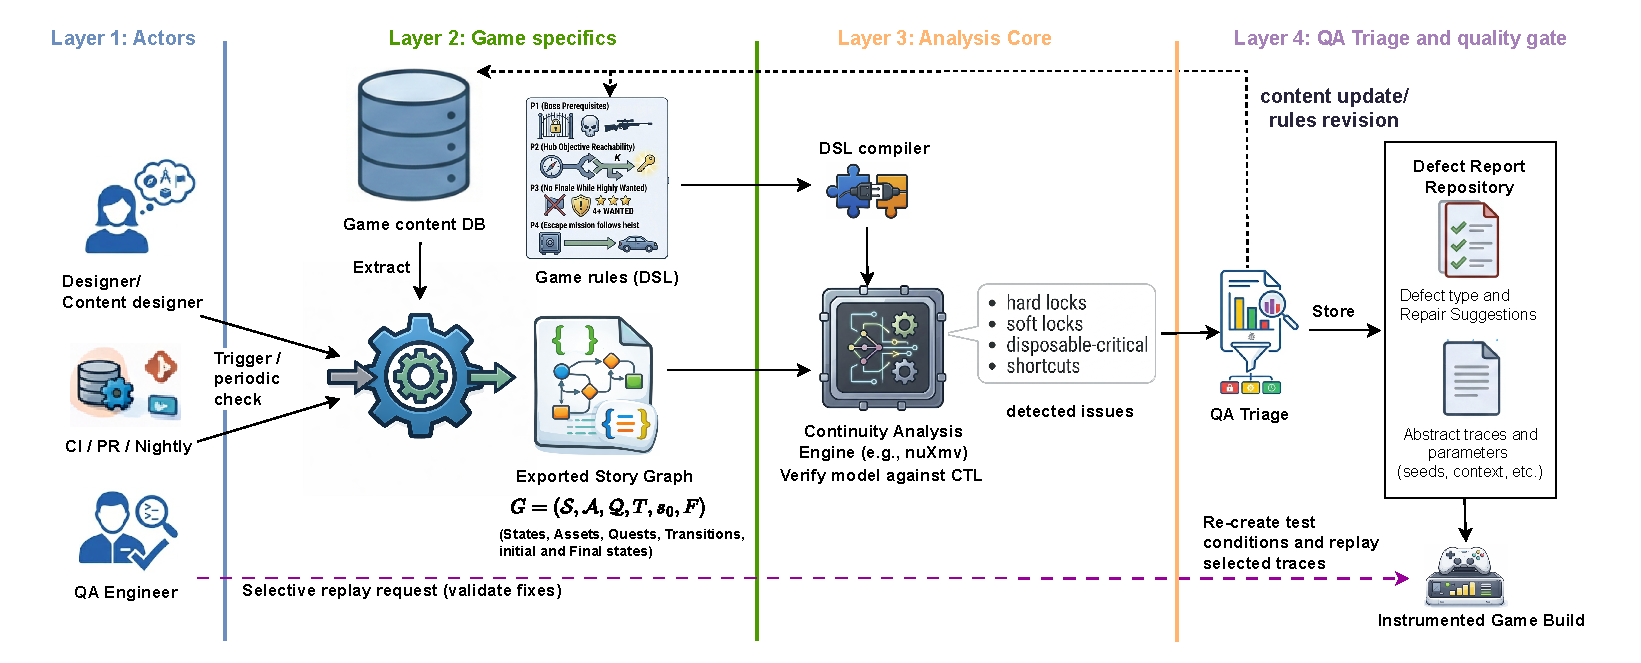
\includegraphics[width=\linewidth]{Flow.pdf}
  \caption{Continuity verification workflow. 
Layer~1 represents triggering actors and periodic validation events. 
Layer~2 contains project-specific artefacts, including production metadata and project-authored DSL rules, which are exported into a resource-annotated story graph. 
Layer~3 implements the engine-independent analysis core, comprising DSL compilation, symbolic model construction, CTL-based property checking, and graph-based defect detection over abstract configurations. 
Layer~4 supports QA triage, defect reporting, selective replay of counterexample traces on instrumented builds, and subsequent content or rule revision. 
Dashed links denote secondary loops: (i) a feedback loop from QA triage to content/rule revision and (ii) an optional loop that replays selected counterexample traces on instrumented builds.}
  \label{fig:framework-overview}
\end{figure*}

\subsection{Story-Graph Model and Annotations}
\label{sec:model}

The chapter-level abstraction models story progression as a finite-state
transition system enriched with a resource summary
\cite{MorenoGer2009ModelCheckingAdventure,Thompson2015IntervalTemporalLogicStories,Lima2023PlotStructureNarratives}.
In narrative games, resources include items, skills, and progression
flags; in this abstraction, these are treated uniformly as \emph{assets}.

\subsubsection{Resource-Annotated Story Graph}

A story graph is represented as a tuple
\(
G = (\States, \Assets, \Quests, T, s_0, F),
\)
where $\States$ is a finite set of abstract story states (e.g.,
missions, hubs, cutscenes), $\Assets$ is a finite set of asset
identifiers (items, skills, flags), and $\Quests$ is a finite set of
quest identifiers partitioned into main-story quests $\MainQ$ and side
quests $\SideQ$. The transition relation
$T \subseteq \States \times \Gamma \times \States$ contains labelled
moves between story states. A tuple $(s_i,\gamma,s_{i+1}) \in T$ denotes
a possible move from $s_i$ to $s_{i+1}$ when the guard encoded by
$\gamma$ holds. The initial story state for the chapter is $s_0$, and
$F$ is the set of completion states.

Each transition label $\gamma \in \Gamma$ encodes (i) a precondition
predicate $\mathit{pre}(\gamma)$ over the current story state and asset
summary, and (ii) an effect function $\mathit{eff}(\gamma)$ that updates
the asset summary after the transition is taken, such as setting flags,
granting items, or consuming items.

A \emph{configuration} summarises a playthrough state as
\begin{equation}
\sigma = (s, A_\sigma),
\quad\text{with}\quad
s \in \States,\; A_\sigma \subseteq \Assets,
\end{equation}
where $A_\sigma$ denotes assets currently held or activated. The set of
configurations reachable from the initial configuration is denoted
$\Sigma$. The abstraction omits low-level engine state, such as spatial position,
animation state, and combat AI. The targeted continuity defects are
defined in terms of access to content and required resources.

\subsubsection{Asset Categories and Mandatory Story States}

Asset metadata is enriched with a lightweight classification to
distinguish recoverable from irreversible resource losses:

\begin{itemize}[leftmargin=1.3em]
  \item \emph{Unique} assets represent non-replicable resources (e.g.,
        single-instance mission items).
  \item \emph{Replenishable} assets can be reacquired through gameplay
        loops (e.g., currency, consumables).
  \item \emph{Transformable} assets are consumed and replaced by other
        assets (e.g., fragments converted into a permanent unlock).
\end{itemize}

A subset of story states $\mathcal{M} \subseteq \States$ is marked as
\emph{mandatory story states}. These states represent narrative
milestones for which explicit prerequisites are meaningful, such as arc
transitions or boss encounters. Each mandatory story state
$X \in \mathcal{M}$ is annotated with required assets
$\mathit{Req}_X \subseteq \Assets$ and, optionally, recommended assets
$\mathit{Rec}_X \subseteq \Assets$. In production pipelines, these
annotations can be derived from existing fields such as mission
prerequisites, unlock conditions, and recommended loadouts.

\subsubsection{Quests, Support Relations, and Repair Suggestions}

Quests are separate content objects associated with progression, while
story states are nodes in the progression graph. A quest may unlock a
story state, require assets before it becomes available, or grant assets
on completion. Each quest $q \in \Quests$ is associated with a role
$\mathit{role}(q)\in\{\texttt{main},\texttt{side}\}$, a precondition
predicate $\mathit{pre}(q)$ describing availability, and a reward set
$\mathit{rew}(q)\subseteq\Assets$ describing assets granted on
completion.
Side content frequently supports later mandatory story states. A support
relation maps assets to side quests that can provide them or provide
declared substitutes. For a configuration $\sigma=(X,A_\sigma)$ at a
mandatory story state $X$, missing prerequisites are defined as
\begin{equation}
M_X(\sigma) = \{ a \in \mathit{Req}_X \mid a \notin A_\sigma \}.
\end{equation}

A \emph{repair suggestion} is a set of side quests whose exported reward
sets cover $M_X(\sigma)$ under the acquisition model. Suggestions are
\emph{advisory}: they provide candidate content-level interventions,
such as preserving availability of supporting quests before a mandatory
story state or adding an alternative acquisition route for a required
asset. They are not automated fixes.

\subsection{Defect Taxonomy and Pipeline Interfaces}
\label{sec:taxonomy-and-interfaces}

The analysis targets continuity defects expressed over the configuration
space induced by the story-graph model (Section~\ref{sec:model}). The
taxonomy is aligned with recurring failure modes in narrative progression
testing \cite{Coppola2024CoverageMetrics,Coppola2024KnowYourBugs}. This
subsection also defines the minimal interfaces required to connect the
analysis core to project-specific content pipelines and engine builds.

\subsubsection{Continuity Defect Classes}
\label{sec:defect-classes}

Let $F \subseteq \States$ denote completion states. A \emph{completion
configuration} is any configuration whose story state lies in $F$. The
following defect classes use familiar game QA terminology, but each class
is defined below as a property over the exported progression model.

\noindent\emph{Hard locks.}
A configuration is hard-locked when it is reachable from the initial
configuration and no completion configuration is reachable from it.
Hard locks represent irreversible progression dead ends, such as missing
a required unlock or losing access to a mandatory route.

\noindent\emph{Soft locks.}
A soft lock denotes a reachable configuration from which completion
remains possible, but only through a recovery path whose cost exceeds a
threshold $\theta$. Cost is instantiated by transition count or by a
project-defined proxy, such as the number of quest steps or required
objectives. In the evaluation, cost is transition count and $\theta$ is
fixed per chapter slice.

\noindent\emph{Disposable-critical-resource defects.}
Disposable-critical defects arise when a unique or otherwise critical
asset is lost irreversibly, while a mandatory story state requiring that
asset can still be reached. This class
covers cases such as selling or consuming a single-instance key item, or
triggering a one-time resource transfer that eliminates the intended
route to a required capability.

\noindent\emph{Shortcut defects.}
A shortcut defect occurs when a mandatory story state becomes reachable
in a configuration that violates its required-asset set. This class
captures unintended sequence breaks, such as reaching an arc transition
without completing prerequisites or entering a boss encounter without a
required tool. This also covers cases where one path into mandatory content checks the
required assets, but another path reaches the same content without that
check.

\subsubsection{Engine-Independent Architecture}
\label{sec:architecture}

Project-specific concerns are isolated behind two adapters:

\begin{itemize}[leftmargin=1.3em]
  \item \texttt{StoryGraphExtractor}, which maps production content
        sources (databases, authoring tools, or engine-side metadata)
        into the common story-graph representation, including asset
        annotations and mandatory story state requirements;
  \item \texttt{ReplayHarness}, which interprets abstract traces as
        executable actions on a game build and reports whether the
        expected configuration is reached.
\end{itemize}

The analysis core consumes the exported story graph, the DSL rule set,
and optionally an identifier-to-action mapping for replay. It assumes no
access to internal engine representations beyond what is exposed through
extraction and replay.

\noindent\textbf{Extraction inputs.}
At minimum, extraction requires (i) a set of story states, (ii) a
dependency or transition structure, and (iii) resource effects governing
progression. In production settings, these inputs typically correspond
to mission definitions, prerequisite fields, quest reward relations, and
progression flag updates. When scripted transitions are not encoded in
structured metadata, the exported model can incorporate explicit
overrides authored for analysis or remain conservative by omitting such
edges.

\subsubsection{Export Schema}
\label{sec:export-schema}

Extracted story graphs are serialised into an engine-independent JSON
representation that records: (i) story states and tags, (ii) assets and
their categories, (iii) quest roles and rewards, (iv) mandatory story
states with required and recommended assets, (v) transitions with
preconditions and effects, and (vi) initial and completion states. The
export format serves as an interchange contract between project adapters
and the analysis core (Listing~\ref{lst:json-schema}).

\begin{figure*}[htbp]
\begin{lstlisting}[
style=UBListingStory,
caption={Excerpt of an engine-independent JSON export capturing story states, assets, quests, mandatory story states, and guarded transitions for a chapter-sized slice. The export format acts as an interchange contract between project-specific extractors and the analysis core.},
label={lst:json-schema}]
{
  "states":          [ { "id": "M7_Boss", "kind": "mission", "tags": ["mandatory"] }, ... ],
  "assets":          [ { "id": "SniperRifle", "category": "unique", "support_quests": ["Q3_SideSniper"] }, ... ],
  "quests":          [ { "id": "Q3_SideSniper", "role": "side", "rewards": ["SniperRifle"] }, ... ],
  "mandatory_story_states": [ { "state": "M7_Boss", "required": ["SniperRifle"], "recommended": ["ArmorUpgrade_Lv2","DodgeAbility"] }, ... ],
  "transitions": [
    { "from": "CityHub",      "to": "M3_BankHeist",
      "pre": ["HasFlag('StoryObjectiveFlag')"],
      "eff": ["AddFlag('HeistStarted')"] },
    { "from": "M3_BankHeist", "to": "M7_Boss",
      "pre": ["HasAsset('SniperRifle')"],
      "eff": ["AddFlag('FinaleUnlocked')"] },
    ...
  ],
  "initial_state":     "M1_Intro",
  "completion_states": ["M7_Boss"]
}
\end{lstlisting}
\end{figure*}

\subsubsection{Verification Model Construction}
\label{sec:json-to-model}

The JSON export is interpreted as a declarative description of a finite
transition system suitable for property checking. Model construction
introduces a finite-domain variable for the control state, boolean or
finite-domain variables for asset predicates, and guarded updates derived
from transition preconditions and effects. Initial and completion
conditions are derived directly from \texttt{initial\_state} and
\texttt{completion\_states} fields.

\noindent\emph{Extraction procedures.}
Extraction is a project-specific step handled by
\texttt{StoryGraphExtractor}. In database-backed pipelines, extraction
typically joins mission tables, prerequisite fields, quest definitions,
and reward relations to build states, assets, and guarded transitions.
In engine-authored pipelines, extraction traverses authoring artefacts
(e.g., ScriptableObjects in Unity) at editor time.

\subsection{Requirements DSL}
\label{sec:dsl}

Continuity expectations are expressed as rules in a small
domain-specific language (DSL) evaluated over the exported story model. 
Rules are authored using narrative progression concepts
(missions, hubs, assets) rather than verification-model internals.

\subsubsection{Rule Structure}

Listing~\ref{lst:DSLrule} shows the general structure of a continuity rule.

\begin{lstlisting}[style=UBListingDSL,
                   numbers=none,
                   basicstyle=\ttfamily\scriptsize,
                   caption={General structure of a continuity rule.},
                   label={lst:DSLrule},
                   linewidth=0.98\linewidth]
RULE <Name>:
  WHEN <Trigger>
  REQUIRE <Constraint>
  [WITHIN <K> STEPS]
\end{lstlisting}

\texttt{Trigger} denotes a story-level event such as entering a mission
or hub, completing a mission, or reaching a tagged state.
\texttt{Constraint} is a predicate over the current abstract control
state and resource summary, such as possession of an asset, satisfaction
of a prerequisite condition, or a boolean abstraction of a numeric
condition. The optional \texttt{WITHIN K STEPS} clause expresses a
bounded reachability obligation over exported transitions, where the
bound counts story transitions.

\subsubsection{Examples and Property Interpretation}

\begin{lstlisting}[style=UBListingDSL,float=htbp,
                   caption={Representative continuity rules in the DSL,
together with their temporal-property interpretations (P1--P4). Bounded
reachability uses a step bound $K$ over exported story transitions. $AF^{\le K}$ denotes a step-bounded eventuality, encoded by bounded unrolling up to depth $K$ (Section~\ref{sec:algorithms}).},
                   label={lst:dsl-rules}]                   
-- P1: Boss prerequisites must be met.
RULE BossPrereqsMet:
  WHEN EnterMission("M7_Boss")
  REQUIRE HasAsset("SniperRifle")

P1 BossPrereqsMet =
  AG( atState(M7_Boss) -> has(SniperRifle) )

-- P2: Hub objective is reachable within K steps.
RULE HubObjectiveReachable:
  WHEN EnterHub("CityHub")
  REQUIRE HasFlag("StoryObjectiveFlag")
  WITHIN K STEPS

P2 HubObjectiveReachable =
 AG(atState(CityHub)->AF<=K has(StoryObjectiveFlag))

-- P3: Finale cannot complete if highly wanted.
RULE NoFinalWhileHighlyWanted:
  WHEN CompleteMission("M_Final")
  REQUIRE WantedLevelBelow(4)

P3 NoFinalWhileHighlyWanted =
  AG( completed(M_Final) -> !wantedLevelGE4 )

-- P4: Escape mission must follow the heist.
RULE EscapeImmediatelyAfterHeist:
  WHEN CompleteMission("M3_BankHeist")
  REQUIRE NextStateIs("M3_Escape")

P4 EscapeImmediatelyAfterHeist =
  AG(completed(M3_BankHeist)->AX atState(M3_Escape))
\end{lstlisting}

In Listing~\ref{lst:dsl-rules}, P1 encodes a prerequisite invariant: entry into a designated encounter
is inconsistent when a required asset is not present. P2 encodes a
bounded progress obligation: after reaching a hub state, the primary
objective flag must become achievable within at most $K$ story
transitions. P3 encodes a completion constraint: finale completion is
disallowed under an abstracted ``high wanted level'' condition. P4
encodes an ordering constraint: completion of a mission must be followed
immediately by a designated successor state.

Triggers such as \texttt{EnterHub} and \texttt{EnterMission} are
evaluated over exported transitions, and bounded obligations start at
the first entry into the trigger state along each path. Numeric
quantities are handled via export-time boolean abstractions, such as
\texttt{WantedLevelBelow(4)}, to avoid unbounded numeric domains.

\subsection{Analysis Pipeline and Algorithms}
\label{sec:algorithms}

The analysis phase combines (i) property checking for DSL rules and
(ii) graph-based detection of global continuity patterns. Property
checking captures specification-driven constraints, such as prerequisites
and bounded progress. Graph procedures capture reachability and
resource-sensitive defect regions, such as hard locks, soft locks,
disposable-critical losses, and shortcut states.

\subsubsection{Abstract Configuration Space}

The concrete configuration set $\Sigma$ can grow combinatorially with
asset combinations. The procedures therefore operate over
\emph{abstract configurations} that preserve (i) the current story state
$s \in \States$ and (ii) a projection of the asset set to the subset of
$\Assets$ referenced by mandatory story state requirements or DSL
predicates. Two configurations with the same story state and identical
projection are treated as equivalent for exploration and defect
detection. This abstraction preserves the information needed for the defect classes
targeted here, because reported violations depend on prerequisite assets
and reachability over exported transitions.

\subsubsection{Property Checking for DSL Rules}

Each DSL rule is compiled into a temporal property over the symbolic
verification model derived from the JSON export
(Section~\ref{sec:json-to-model}). The resulting properties follow
standard schemas \cite{Clarke2018ModelChecking2e}:

\begin{itemize}[leftmargin=1.3em]
  \item \emph{Prerequisite invariants} ensuring that designated states
        are not reached without required assets.
  \item \emph{Bounded progress obligations} requiring that a condition
        becomes achievable within a bounded number of story transitions
        after a trigger.
  \item \emph{Ordering constraints} restricting allowed successors or
        enforcing immediate follow-up states after a completion event.
\end{itemize}

Violations produce counterexample traces at the level of story-state and
asset predicates. These traces are normalised into an engine-independent
trace format for replay (Section~\ref{sec:trace-replay}).

Rules without a \texttt{WITHIN} clause are compiled to CTL properties and
model-checked using NuSMV~\cite{CimattiCGGPRST02}. Step-bounded
obligations introduced by \texttt{WITHIN K STEPS} are encoded by
unrolling exported story transitions up to depth $K$. The encoding uses
auxiliary variables that track the remaining bound and reduces the check
to CTL model checking over a finite extended model. Concretely, an
auxiliary step counter $(0\dots K)$ is updated on each exported
transition, and the obligation is checked as a standard CTL eventuality
over the extended model.

\subsubsection{Graph-Based Detection of Global Defect Patterns}

The defect classes defined in Section~\ref{sec:defect-classes} are
detected by exploring the abstract configuration graph induced by the
exported transition relation and asset effects.

\noindent\emph{Hard-lock detection.}
Let $R_{\mathrm{init}}$ be the configurations reachable from the initial
configuration, and let $R_F$ be the configurations from which some
completion configuration can still be reached. Hard-lock candidates are
then $H = R_{\mathrm{init}} \setminus R_F$.
That is, a hard-lock candidate is reachable during play, but no completion
state remains reachable from it.

\noindent\emph{Soft-lock detection.}
Let $d(\sigma,F)$ be the minimum recovery cost from configuration
$\sigma$ to any completion configuration, defined only when completion
remains reachable. Soft-lock candidates are
$S = \{ \sigma \in R_{\mathrm{init}} \cap R_F \mid d(\sigma,F) > \theta \}$.
In the evaluation, cost is measured as transition count and $\theta$ is fixed per slice.

\noindent\emph{Disposable-critical-resource detection.}
Let $\Assets_{\mathrm{crit}} \subseteq \Assets$ denote the set of unique
or otherwise critical assets. For each critical asset
$a \in \Assets_{\mathrm{crit}}$, the analysis computes the configurations
from which $a$ can still be recovered under the exported acquisition
model. A transition $\sigma \rightarrow \sigma'$, with
$\sigma'=(s',A_{\sigma'})$, is reported when it removes $a$ from the
current asset set, i.e., $a \in A_\sigma$ and $a \notin A_{\sigma'}$,
and moves from a configuration where recovery is possible to one where
recovery is no longer possible, while a mandatory story state requiring
$a$ remains reachable.

\noindent\emph{Shortcut detection.}
Algorithm~\ref{alg:shortcut} performs a worklist exploration over
abstract configurations and reports reachable mandatory story states
whose required constraints are missing.

\begin{algorithm}[t]
  \caption{FindShortcutBugs$(G)$}
  \label{alg:shortcut}
  \begin{algorithmic}[1]
    \STATE $B \gets \emptyset$
    \STATE Initialise a worklist $W$ with the initial configuration $\sigma_0$
    \STATE Maintain a visited set over abstract configurations
    \WHILE{$W$ not empty}
      \STATE pop $\sigma = (s, A_\sigma)$ from $W$
      \IF{abstract configuration of $\sigma$ already visited}
        \STATE \textbf{continue}
      \ENDIF
      \STATE mark abstract configuration of $\sigma$ as visited
      \IF{$s \in \mathcal{M}$ \textbf{ and } $\mathit{Req}_s \nsubseteq A_\sigma$}
        \STATE add $\sigma$ to $B$
      \ENDIF
      \FORALL{enabled transitions $\sigma \rightarrow \sigma'$}
        \STATE add $\sigma'$ to $W$
      \ENDFOR
    \ENDWHILE
    \RETURN $B$
  \end{algorithmic}
\end{algorithm}

\noindent\textbf{Complexity.}
For the transition-count costs used in the evaluation, each exploration
procedure visits each abstract configuration at most once and processes
outgoing transitions of visited nodes. The graph procedures run in
$O(|\Sigma_a| + |T_a|)$, where $\Sigma_a$ and $T_a$ denote the abstract
configuration set and its induced transition relation.

\subsection{Trace Generation and Engine Replay}
\label{sec:trace-replay}

Continuity violations are converted into executable test cases through
trace generation and replay. Replay checks whether reported defects
correspond to observable runtime behaviour rather than modelling
artefacts \cite{Shirzadeh2022Experience, Shirzadehhajimahmood2021RobustGameTesting}.

\subsubsection{Engine-Independent Trace Representation}

Each violation is associated with an abstract counterexample trace
\begin{equation}
\pi = \langle \alpha_0, \alpha_1, \dots, \alpha_n \rangle,
\end{equation}
where each abstract action $\alpha_k$ encodes (i) a target story-state
identifier, (ii) an action type (e.g., enter mission, complete objective,
unlock hub, acquire asset), and (iii) optional parameters (e.g., mission
ID, asset ID).

Traces are serialised in a JSON-based format that references only
identifiers present in the exported story graph. The representation is
independent of input devices, UI layouts, and scripting languages, and
can be interpreted by different replay mechanisms in prototype and
production environments.

\subsubsection{Replay Harness Interface}

Replay is implemented through the \texttt{ReplayHarness} adapter, which
interprets abstract actions against a concrete build. The adapter:

\begin{enumerate}[leftmargin=1.3em]
  \item resets the build to a known initial save state,
  \item maps each abstract action to engine-level calls or scripted
        interactions,
  \item executes the action sequence deterministically,
  \item reads back relevant progression state (e.g., quest log,
        inventory, flags),
  \item compares the observed configuration with the expected
        configuration derived from the analysis.
\end{enumerate}

Replay success indicates that the abstract counterexample corresponds to
a reproducible in-engine scenario. Replay failure usually indicates either
a harness limitation or a mismatch between exported metadata and runtime
behaviour, such as a missing scripted transition or a mismatched
identifier. In production settings, replay is applied selectively rather than to every
reported violation. Its role is to connect a violated rule or defect class
to a trace and, when available, to runtime artefacts
such as logs or screenshots.

%%%%%%%%%%%%%%%%%%%%%%%%%%%%%%%%%%%%%%%%%%%%%%%%%%%%%%%%%
\section{Evaluation}
\label{sec:evaluation}

The evaluation examines two commercial quest-driven games and an
open-source Unity prototype. It assesses detection coverage, analysis
cost, replay feasibility, and transfer effort across projects.

\subsection{Experimental Setup}
\label{sec:setup}

The checker consumes exported JSON story graphs and DSL rule files. It
builds a finite-domain verification model from guarded updates and
evaluates four analysis configurations: structural reachability (SR),
asset-agnostic reachability with quests (AQ), resource-aware reachability
without DSL rules (RA), and symbolic continuity (SC). SC combines DSL
property checking with graph procedures over abstract configurations
(Section~\ref{sec:algorithms}).

In the evaluated pipelines, analysis runs one chapter at a time on
content-branch updates that modify quest, item, or prerequisite
structure. Slices are checked offline and triaged by defect class,
violated rule or pattern, and counterexample trace. Replay is applied
selectively for build-level confirmation.

\noindent\textbf{Baselines.}
The evaluation uses three diagnostic baselines: structural reachability
(SR), asset-agnostic reachability with quests (AQ), and resource-aware
reachability without DSL rules (RA).
These are used to isolate the added value of the
proposed method over simpler checks of graph structure, quest structure,
and resource evolution. These baselines are inspired by common
content-validation practice and by abstractions used in prior work on
automated and model-based game testing
\cite{Shirzadeh2022Experience,Politowski2021SurveyVGT,Prasetya2025MBTGames,Iftikhar2015MBTPlatformGames}.
Replay is reported only for SC because the replay harness consumes SC
counterexample traces, whereas the baselines report diagnostic anomalies
rather than replay-ready violations.


\textit{Structural reachability (SR).}
SR analyses the directed graph over story states and transitions while
ignoring quests, assets, and DSL rules. It reports disconnected regions,
dead ends, and reachability anomalies, but does not represent missing
prerequisites or irreversible resource loss.

\textit{Asset-agnostic reachability with quests (AQ).}
AQ extends SR with quest nodes and quest-to-state links derived from
quest availability. It highlights unexpected predecessors and quest-chain
discontinuities, but does not enforce per-state requirements or asset
consistency.

\textit{Resource-aware reachability without DSL rules (RA).}
RA explores the abstract configuration graph induced by asset
preconditions and effects, but does not check authored DSL rules or
mandatory-state requirement annotations. It can expose hard locks and
some soft locks when they are visible through resource-sensitive
reachability. It can also surface limited disposable-critical or
shortcut-like symptoms when they manifest as reachability anomalies, but
it does not directly check the requirements that define these classes.


The proposed approach is denoted \textbf{SC} (symbolic continuity). It
uses the exported story model, mandatory story state requirements, and DSL
properties. It also emits counterexample traces and supports optional
replay.

Across case studies, the workflow follows a common sequence:

\begin{enumerate}[leftmargin=1.3em]
  \item Export a chapter-level story graph, asset annotations, and
        mandatory story state requirements in the JSON schema
        (Section~\ref{sec:export-schema}).
  \item Load the continuity DSL rule set (Section~\ref{sec:dsl}).
  \item Run SR, AQ, RA, and SC on the exported slice.
  \item Generate a report containing defect class, violated rule or
        pattern, an abstract counterexample trace, and optional repair
        suggestions.
  \item Replay selected traces on a build and attach runtime artefacts
        (logs and screenshots) when replay is successful.
\end{enumerate}


\subsection{Case Study Context and Ground Truth}
\label{sec:case-studies}

Ground truth combines historical issues with seeded defects targeting
specific continuity classes. For the industrial cases, issue counts are
aggregated across the evaluated content-update variants for each chapter
slice.

\noindent\textbf{Case A: \emph{Gangstar New Orleans}.}

A chapter slice is exported from a commercial open-world mobile
title.\footnote{\url{https://www.gameloft.com/game/gangstar-new-orleans}}
The exported model contains 61 abstract states (missions, hubs, and
cutscenes), 95 assets (items, skills, and progression flags), 43 quests
(19 main arcs and 24 side missions), and 184 guarded transitions. The
analysis uses structured progression metadata and reward/prerequisite
fields; engine source code and runtime AI behaviour are not part of the
verification model.

Historical issues are derived from internal issue-tracker
records and design notes for the exported slice. A total of 140 issues are
labelled continuity-related by content owners, including unintended sequence
breaks, missing prerequisites, and irreversible loss of required items.
To exercise all defect classes, 80 additional defects are seeded by
controlled modifications to content metadata, such as removing fallback
transitions, reclassifying a required item as unique/consumable, or
loosening a prerequisite. This yields 220 ground-truth entries in total.

\noindent\textbf{Case B: \emph{Carmen Sandiego}.}
A second chapter slice is exported from a narrative-driven detective
adventure with capability gating.\footnote{\url{https://carmensandiego-game.com/}}
The exported model contains 48 abstract states, 72 assets, 33 quests
(15 main and 18 side), and 143 transitions. As in case A, analysis uses
structured progression metadata and reward/prerequisite fields.

Ground truth for the chapter slice comprises 100 historical continuity
issues documented internally, such as reaching a clue-gated scene without an intended evidence flag, losing access to a one-time travel token, or
bypassing a tutorial gate. Eighty additional seeded defects are
introduced to exercise disposable-critical and soft-lock scenarios, for a
total of 180 ground-truth entries.

\noindent\textbf{Open-source Unity prototype.}
The prototype implements a chapter-sized scenario used for running
examples and replication. The exported model contains 25 states, 40
assets, 18 quests (8 main and 10 side), and 80 transitions. All 28 defects are seeded by construction: eight hard locks, eight soft
locks, six disposable-critical defects, and six shortcut defects.

Table~\ref{tab:ground-truth-composition} summarises the composition of
the ground truth. Historical issues assess whether the approach recovers
continuity problems observed in production artefacts or QA records.
Seeded defects exercise specific defect classes under controlled
conditions. The two sources are reported separately because they support
different claims: historical issues provide practical relevance, while seeded defects provide controlled coverage of the taxonomy.

\begin{table}[t]
  \caption{Ground-truth composition by case study.}
  \label{tab:ground-truth-composition}
  \centering
  \begin{tabular}{lccc}
    \toprule
    Case study & Historical & Seeded & Total \\
    \midrule
    Gangstar New Orleans & 140 & 80  & 220 \\
    Carmen Sandiego      & 100 & 80  & 180 \\
    Unity prototype      & 0   & 28  & 28  \\
    \bottomrule
  \end{tabular}
\end{table}

\noindent\textbf{Labelling procedure.}
For each setting, each report is labelled as a true positive,
false positive, or duplicate relative to the known/seeded defect set and,
for the industrial slices, content-owner judgement. Reports are treated
as duplicates when they map to the same underlying defect after
inspection of the violating mandatory story state and the missing or
mis-specified prerequisite resources. For SC reports, replay is attempted
when a trace can be mapped by the harness, and replay success is
recorded.

All experiments were run on a workstation-class desktop equipped with an
AMD Ryzen-class CPU (24 cores) and 64\,GB RAM. Reported
analysis time includes model construction and checking, including trace
generation; export and replay time are excluded.

\noindent\textbf{Evaluation measures.}
The evaluation reports the following measures:

\begin{itemize}[leftmargin=1.3em]
\item \textit{Detection rate}: number of ground-truth entries correctly
        reported, stratified by defect class.
\item \textit{False positives}: reports not corresponding to
        ground truth or accepted design concerns.
  \item \textit{Analysis time}: wall-clock time for model construction,
        analysis, checking, and trace generation; export and replay are excluded.
  \item \textit{Replay success rate (SC)}: fraction of SC counterexamples
        that replay to completion and reproduce the expected configuration.
  \item \textit{Trace length (SC)}: number of steps in replayed traces.
\end{itemize}

These measures separate detection quality from operational usefulness:
triage noise, checker cost, and the effort needed to inspect replayable
violations.

\subsection{Results: Defect Detection}
\label{sec:results-detection}

Tables~\ref{tab:results-gno}--\ref{tab:results-proto} report detection
results by defect class. The totals combine historical and seeded
defects, while Table~\ref{tab:ground-truth-composition} reports the
source composition of the ground truth. This distinction is important:
historical issues assess recovery of known production-relevant
defects, whereas seeded defects assess controlled coverage of the defect
taxonomy.

SR and AQ recover a subset of hard locks and structural anomalies, but
they do not represent asset evolution, authored requirements, bounded
progress obligations, or irreversible resource loss. RA improves coverage for defects that depend on resource preconditions or
effects visible in the exported graph, although it does not subsume all
quest-structure diagnostics captured by AQ. Its remaining misses occur mainly when the defect depends on authored mandatory-state requirements,
critical-resource annotations, or bounded obligations expressed in the
DSL. SC adds these requirements and therefore increases coverage for soft
locks, disposable-critical defects, and shortcuts.

Analysis remained within tens of seconds per exported content-update
variant (Table~\ref{tab:cost}), and replay supports build-level
reproduction for most SC-detected issues in the industrial slices
(Section~\ref{sec:replay-results}). The SC runtime is not determined only
by the number of story states and transitions; it also depends on the
number of DSL rules, bounded checks, and generated counterexample traces.

\begin{table}[t]
  \caption{Detection results on \emph{Gangstar New Orleans} (industrial case A).}
  \label{tab:results-gno}
  \centering
  \scriptsize
  \setlength{\tabcolsep}{3pt}
  \begin{tabular}{lcccccc}
    \toprule
    Category & \# & SR & AQ & RA & \textbf{SC} & SC Replay \\
    \midrule
    Hard lock           & 60 & 41/60 & 49/60 & 58/60 & \textbf{60/60} & 60/60 \\
    Soft lock           & 80 & 12/80 & 33/80 & 52/80 & \textbf{63/80} & 63/63 \\
    Disposable-critical & 40 & 0/40  & 2/40  & 11/40 & \textbf{29/40} & 29/29 \\
    Shortcut            & 40 & 18/40 & 21/40 & 24/40 & \textbf{38/40} & 28/38 \\
    \midrule
    False positives     & -- & 63    & 48    & 42    & \textbf{27}    & --    \\
    \bottomrule
  \end{tabular}
\end{table}

\begin{table}[t]
  \caption{Detection results on \emph{Carmen Sandiego} (industrial case B).}
  \label{tab:results-carmen}
  \centering
  \scriptsize
  \setlength{\tabcolsep}{3pt}
  \begin{tabular}{lcccccc}
    \toprule
    Category & \# & SR & AQ & RA & \textbf{SC} & SC Replay \\
    \midrule
    Hard lock           & 50 & 29/50 & 41/50 & 48/50 & \textbf{50/50} & 50/50 \\
    Soft lock           & 50 & 9/50  & 22/50 & 31/50 & \textbf{42/50} & 42/42 \\
    Disposable-critical & 40 & 0/40  & 1/40  & 13/40 & \textbf{32/40} & 32/32 \\
    Shortcut            & 40 & 19/40 & 22/40 & 21/40 & \textbf{31/40} & 22/31 \\
    \midrule
    False positives     & -- & 38    & 43    & 28    & \textbf{21}    & --    \\
    \bottomrule
  \end{tabular}
\end{table}

\begin{table}[t]
  \caption{Detection results on the Unity prototype.}
  \label{tab:results-proto}
  \centering
  \scriptsize
  \setlength{\tabcolsep}{3pt}
  \begin{tabular}{lcccccc}
    \toprule
    Category & \# & SR & AQ & RA & \textbf{SC} & SC Replay \\
    \midrule
    Hard lock           & 8 & 3/8 & 5/8 & 7/8 & \textbf{8/8} & 8/8 \\
    Soft lock           & 8 & 1/8 & 3/8 & 5/8 & \textbf{7/8} & 7/7 \\
    Disposable-critical & 6 & 0/6 & 0/6 & 3/6 & \textbf{6/6} & 6/6 \\
    Shortcut            & 6 & 2/6 & 3/6 & 2/6 & \textbf{5/6} & 5/5 \\
    \midrule
    False positives     & -- & 5   & 9   & 4   & \textbf{3}   & --  \\
    \bottomrule
  \end{tabular}
\end{table}

\subsection{Operational Cost and Pipeline Suitability}
\label{sec:cost}

Table~\ref{tab:cost} reports analysis time per exported content-update
variant; export and replay are excluded. RA incurs additional cost over SR and
AQ because it explores asset-sensitive configurations. SC adds DSL
property checking and trace generation on top of resource-aware
exploration. Across the industrial slices, peak memory usage remains below
200\,MB because analysis is performed on projected abstract
configurations rather than on the full asset powerset. Runtime is primarily influenced by the number of exported
states and transitions and by the number of relevant asset predicates
induced by mandatory story state requirements and DSL rules. The gap
between RA and SC reflects the additional cost of compiling and checking
authored continuity rules, beyond exploring the resource-sensitive
configuration graph.

\begin{table}[t]
  \caption{Analysis time (seconds) per exported content-update variant, excluding export and replay.}
  \label{tab:cost}
  \centering
  \begin{tabular}{lcccc}
    \toprule
    Case study & SR & AQ & RA & SC \\
    \midrule
    Gangstar New Orleans (A) & 0.8 & 1.1 & 2.7 & 15.5 \\
    Carmen Sandiego (B)      & 0.6 & 0.9 & 2.0 & 23.7 \\
    Unity prototype          & 0.3 & 0.4 & 0.6 & 7.9 \\
    \bottomrule
  \end{tabular}
\end{table}



\subsection{Replay Feasibility and Triage Value}
\label{sec:replay-results}

Replay is attempted for SC-detected reports that yield a trace and have a
defined harness mapping. In case A, 180 of 190 SC-detected reports replay successfully (95\%); the remaining failures are attributable to harness mapping inconsistencies. In case B, 146 of 155 SC-detected reports replay successfully (94\%); the remaining failures are attributable to
non-deterministic UI timing dependencies in the automation layer. In the
Unity prototype, all 26 SC-detected counterexamples replay successfully
(100\%).

Trace length provides a proxy for inspection effort. In the two
industrial slices, replay traces range from 10 to 38 steps (median 18 in
case A; median 16 in case B). In the prototype, traces range from 9 to
22 steps (median 14). These replay rates indicate that most abstract
counterexamples can be mapped to executable playthroughs in the evaluated
settings.

\subsection{Industrial Adoption Effort and Maintenance}
\label{sec:adoption-effort}

Adoption requires project-specific work at three integration points:
content extraction, rule authoring, and replay. The analysis core is
shared across projects, but each game must provide mappings from its
production content data to the export schema. Replay is not required for
static analysis, but it is useful when counterexamples need to be
confirmed on a build and attached to QA reports.

Table~\ref{tab:adoption-effort} summarises the observed effort in the
prototype and case-study instantiations. The estimates cover the work required to instantiate the workflow on a
representative chapter slice, including implementation, configuration,
and validation of the project-specific adapters and rules. Maintenance
mainly concerns the project-specific layers rather than the analysis core. Extractor mappings must be updated when content schemas
change, for example when prerequisite fields are renamed, quest templates
are split, or reward definitions move to a different authoring table. DSL
rules require review when designers introduce new progression patterns,
change recovery expectations, or rebalance chapter structure. Replay
mappings are more fragile when they depend on UI automation, because menu
flow, timing, and scene loading behaviour can change during production.
Build-level test hooks reduce this maintenance cost, but require
engineering support.


\begin{table}[t]
\caption{Observed project-specific adoption effort.}
\label{tab:adoption-effort}
\centering
\footnotesize
\setlength{\tabcolsep}{3.5pt}
\renewcommand{\arraystretch}{1.08}

\begin{tabularx}{\columnwidth}{@{}
  >{\RaggedRight\arraybackslash}p{1.65cm}
  >{\RaggedRight\arraybackslash}X
  >{\RaggedRight\arraybackslash}p{1.45cm}
@{}}
\toprule
Activity & Required work & Effort \\
         &               & \textit{person-days} \\
\midrule

StoryGraph extractor
& Map mission, prerequisite, reward, flag, and quest fields to the export schema.
& 2--5 \\

\addlinespace[2pt]

DSL rules
& Encode chapter-specific progression constraints, recovery bounds, and ordering expectations.
& 0.5--2 per slice \\

\addlinespace[2pt]

ReplayHarness hooks
& Map abstract trace actions to build-level test APIs or editor hooks.
& 3--8 \\

\addlinespace[2pt]

ReplayHarness UI
& Map abstract trace actions to scripted UI interactions and timing controls.
& 6--12 \\

\addlinespace[2pt]

Triage review
& Inspect violations, merge duplicates, classify false positives, and select traces for replay.
& 5--20 minutes/report \\

\bottomrule
\end{tabularx}
\end{table}

In the evaluated projects, the approach was treated as a chapter-level
validation aid rather than as a replacement for manual QA or exploratory
playtesting. Its practical role is to expose resource-dependent
progression states early and provide replayable traces, allowing QA effort
to focus on selected reports rather than broad manual search.

\subsection{Generalizability and Scalability}
\label{sec:generalizability}

Transfer across projects requires (i) identifiable progression states,
(ii) structured prerequisite and effect fields that can be exported as
guarded transitions, and (iii) resource representations summarised as
assets. These conditions hold in both industrial slices despite genre
differences. Project-specific effort is confined to the export and
automation layers through the \texttt{StoryGraphExtractor} and
\texttt{ReplayHarness} interfaces.

Scalability is dominated by growth in the number of relevant resource
predicates. The implementation mitigates this through projection to
predicates referenced by mandatory story state requirements and DSL
rules, and through chapter-level partitioning. In the evaluated
industrial slices, the full asset sets contain 95 assets (case A) and
72 assets (case B), while the predicate projection retains 28 and 24
predicates, respectively. Under this projection, 3{,}900 abstract
configurations are visited in case A and 2{,}600 in case B, with induced
abstract transition counts of 14{,}200 and 9{,}500.

A sensitivity check that approximately doubles the number of referenced
predicates, by adding additional requirements and rule predicates,
increases the number of visited abstract configurations by approximately
2.1$\times$ and analysis time by approximately 2.4$\times$ on the same
hardware. These observations indicate that, for a fixed chapter size, scalability
depends mainly on how many requirements and rule predicates are authored
for that chapter. They also support chapter-level partitioning as a
practical validation strategy for larger titles.

\subsection{Limitations and Validity Considerations}
\label{sec:threats}

\noindent\emph{Exported model and rule quality.}
The analysis depends on the fidelity of the exported progression model
and on the authored continuity rules. A defect can be missed when its
cause is not present in the export, for example when progression is
changed only in runtime scripts, hidden state updates are not represented
in content metadata, non-standard resource transfers are omitted, or the
issue depends on visual, audio, or timing behaviour. Conversely, false
positives can occur when rules are stricter than the intended design, such
as when a sequence break is intentional. In practice, rules can be kept as
non-blocking checks when design flexibility is intended, and promoted to
blocking checks when the requirement is meant to be enforced.

\noindent\emph{Replay limitations.}
Replay can confirm whether detected issues occur in the game build, but it
cannot recover behaviour that was not exported into the model. Replay also
depends on stable automation hooks. UI-driven replay can be sensitive to
menu flow, loading time, and timing changes. Build-level test APIs or
editor scripting reduce this brittleness when available. In the evaluated
settings, replay failures were mainly caused by harness mapping drift and
UI timing dependencies, rather than by mismatches between the analysis
model and the game build.

\noindent\emph{Evolution and maintenance.}
The evaluation covers chapter-level content updates rather than a
longitudinal live-service deployment. In evolving projects, extractor
mappings, DSL rules, and replay actions must remain aligned with changes
in content schemas, quest templates, balancing thresholds, and automation
hooks. The reported adoption effort therefore reflects initial
integration and chapter-level use; long-term maintenance depends on the
rate of content-pipeline change in each project.

\noindent\emph{Scope of defect types.}
The framework targets resource-based continuity. It does not address
dialogue coherence, narrative consistency beyond resources, multiplayer
progression, or tuning issues independent of assets.

%%%%%%%%%%%%%%%%%%%%%%%%%%%%%%%%%%%%%%%%%%%%%
\section{Conclusions}
\label{sec:conclusion}

Continuity defects in narrative-driven games often arise from the
interaction between story progression and resource evolution. They are
therefore difficult to expose with structure-only checks, because the
problem may depend on missing prerequisites, irreversible resource loss,
or unintended paths into mandatory content.

This paper presented a framework for checking such defects during game
content evolution. The framework exports a resource-annotated story graph
from production metadata, expresses expected continuity behaviour in a
requirements DSL, and analyses the resulting model using graph
exploration and temporal property checking. Reported violations are
translated into engine-independent counterexample traces that can be
replayed on instrumented builds.

The evaluation on two commercial mobile titles and an open-source Unity
prototype shows that the approach detects continuity defects beyond
structural, quest-augmented, and resource-aware diagnostic baselines. It
is particularly useful for defects involving soft locks,
disposable-critical resources, and missing prerequisites at mandatory
story states. The results also show that the workflow can be applied at
chapter level with project-specific extraction and replay adapters.

The approach is intended as a validation aid for story progression
defined through quests, prerequisites, rewards, and progression flags.
Its practical role is to expose resource-dependent progression defects
that are difficult to cover consistently through local testing, and to
provide replayable traces for QA triage. By detecting such cases earlier
in content branches, the workflow can focus QA effort on selected
progression risks rather than broad manual search.

\iffalse
\appendix
\section{Examples}
\subsection{SMV Encoding Sketch}

\begin{lstlisting}[style=UBListing,caption={Sketch of SMV encoding generated from the exported story graph.},label={lst:smv-encoding}]
MODULE main

VAR
  -- Abstract story state (missions, hubs, cutscenes)
  state : {
    M1_Intro, CityHub,
    M3_BankHeist, M3_Escape,
    M6_Rooftop, M7_Boss,
    M9_Ending
  };

  -- Asset and flag predicates from the export
  has_SniperRifle : boolean;
  flag_GateOpened : boolean;
  flag_M7_Visited : boolean;
  StoryObjectiveFlag : boolean;

  -- Example numeric variable for wanted level
  wantedLevel : 0..5;

ASSIGN
  -- Initial configuration from "initial_state"
  init(state) := M1_Intro;
  init(has_SniperRifle) := FALSE;
  init(flag_GateOpened) := FALSE;
  init(flag_M7_Visited) := FALSE;
  init(StoryObjectiveFlag) := FALSE;
  init(wantedLevel) := 0;

  -- Transition relation derived from "transitions"
  next(state) :=
    case
      -- Example transition: M6_Rooftop -> M7_Boss with precondition GateOpened
      state = M6_Rooftop & flag_GateOpened : M7_Boss;

      -- Bank heist completes and immediately leads to escape mission
      state = M3_BankHeist : M3_Escape;

      -- City hub may lead to an objective mission that sets StoryObjectiveFlag
      state = CityHub : CityHub; -- other outgoing edges omitted for brevity

      -- Default: remain in current state if no edge is enabled
      TRUE : state;
    esac;

  -- Simple example of how rewards/effects are encoded
  next(has_SniperRifle) :=
    case
      -- Side quest Q3_SideSniper grants SniperRifle (abstracted here
      -- as a transition into a synthetic state or via a dedicated flag)
      state = CityHub & !has_SniperRifle : TRUE;
      TRUE : has_SniperRifle;
    esac;

  next(flag_GateOpened) :=
    case
      -- Some earlier mission opens the gate (not shown in JSON excerpt)
      -- and the flag persists afterwards
      state = M6_Rooftop : TRUE;
      TRUE : flag_GateOpened;
    esac;

  next(flag_M7_Visited) :=
    case
      state = M7_Boss : TRUE;
      TRUE : flag_M7_Visited;
    esac;

  next(StoryObjectiveFlag) :=
    case
      -- Objective becomes true when a dedicated mission completes
      state = M3_Escape : TRUE;
      TRUE : StoryObjectiveFlag;
    esac;

  next(wantedLevel) :=
    case
      -- Wanted level evolves according to mission type (simplified)
      state = M3_BankHeist : min(wantedLevel + 2, 5);
      state = M3_Escape     : max(wantedLevel - 1, 0);
      TRUE                  : wantedLevel;
    esac;

DEFINE
  -- Propositions used in CTL/LTL properties
  atState_M7_Boss      := state = M7_Boss;
  atState_CityHub      := state = CityHub;
  completed_M_Final    := state = M9_Ending;
  completed_M3_Heist   := state = M3_BankHeist;
  wantedLevelGE4       := wantedLevel >= 4;
  hasSniperRifle       := has_SniperRifle;

-- CTL examples (P1, P3, P4); P2 is checked via BMC with a bound K
CTLSPEC AG (atState_M7_Boss -> hasSniperRifle);

CTLSPEC AG (completed_M_Final -> !wantedLevelGE4);

CTLSPEC AG (completed_M3_Heist -> AX state = M3_Escape);

-- LTL example for hub progress, checked using BMC up to depth K:
-- LTLSPEC G (atState_CityHub -> F StoryObjectiveFlag);
\end{lstlisting}

\fi

\bibliographystyle{IEEEtran}
\bibliography{references}

\end{document}
